\documentclass[ignorenonframetext,hyperref={pdftex,unicode}]{beamer}
%\documentclass[aspectratio=169,ignorenonframetext,hyperref={pdftex,unicode}]{beamer}  %соотношение 16:9

\usepackage{amssymb,amsmath,mathtext} %поддержка формул и русского текста в них
\usepackage{indentfirst,amsfonts} %поддержка русского стиля оформления текста и формул
%\usepackage{makecell,multirow,longtable} %поддержка таблиц занимающих несколько страниц

\usepackage[english,russian]{babel}
\usepackage[T2A]{fontenc}
\usepackage[utf8]{inputenc} %кодировка исходника

% for hyperlinks
\usepackage{hyperref}
% for strike-out text
\usepackage[normalem]{ulem}

\ifpdf
        \usepackage{cmap} % чтобы работал поиск по PDF
        %\usepackage[pdftex]{graphicx}
        \pdfcompresslevel=9 % сжимать PDF
\else
        \usepackage{graphicx}
\fi

\usetheme{Samsolutions} %корпоративная тема

%\setbeamercovered{transparent} %полупрозрачные скрытые элементы

\title{SaM Solutions: Як мы працуем з супольнасцю} %название презентации
%\subtitle{SUBTITLE} %подназвание
\author["Андрэй Захарэвіч"]{Андрэй Захарэвіч\\ andrej@zahar.ws} %автор


\begin{document} %начало документа

\frame{\titlepage} % Создание заглавной страницы


\section{Уступ. Яшчэ раз пра відавочнае.} %названия секций для оглавления

\begin{frame}{Што мы ўжо робім} %новый слайд и его название
	\begin{itemize}
		\item \textbf{LVEE}
			\pause
		\item \textbf{Код у апстрым}
			\pause
		\item \textbf{Публікацыя вучэбных курсаў і абмену ведамі ў кампаніі}
	\end{itemize}
	\begin{center}
 		
\includegraphics[width=\textwidth,height=0.8\textheight,keepaspectratio]{Once_upon_a_time} %так вставляется картинка
	\end{center}
\end{frame} %конец слайда

\section{Што можам зрабіць}
\begin{frame}{Ці ўсё гэта, што мы можам зрабіць карыснага?} 
	Думаю што не. ;)
	\begin{center}
 		
\includegraphics[height=.8\textheight,keepaspectratio]{work-47200_640} 
	\end{center}
\end{frame} %конец слайда

\begin{frame}{Месца і падтрымка для каманд і супольнасцяў}
	\begin{itemize}
		\item \textbf{Месца для сустрэч.}
			\pause
		\item \textbf{І пячэнкі. ;)}
	\end{itemize}
	\begin{center}
		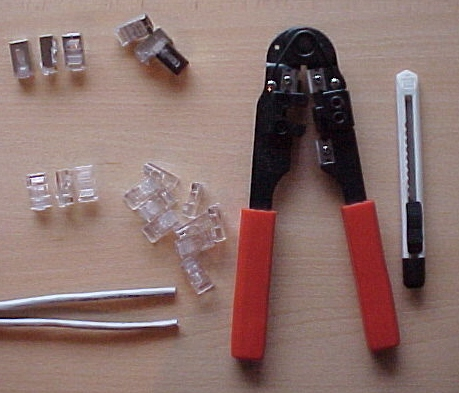
\includegraphics[width=\textwidth,height=0.8\textheight,keepaspectratio]{Utp_diy_tools}
	\end{center}
\end{frame}

		\item \textbf{Лінуксоўкі} 
			\pause

\section{P.S.: Лінуксоўка}
\begin{frame}{Дарэчы, лінуксоўка}
	\begin{center}
		Кожная апошняя субота месяца.\\
		Мінск, Філімонава 15, кабінет 207. (Рухайцеся па стрэлках)
		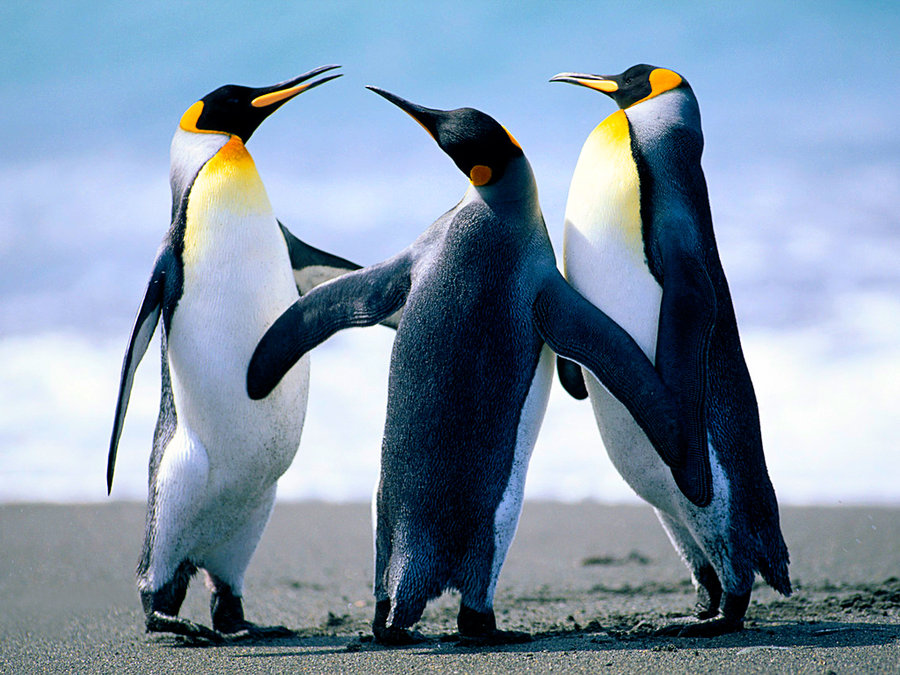
\includegraphics[width=\textwidth,height=0.8\textheight,keepaspectratio]{penguins_by_kyuubidemon98}
	\end{center}
\end{frame}

\section{Прапановы?}
\frame{\finalslide{Прапановы і пытанні?}} %слайд вопросы?

\begin{frame}{Ужытыя малюнкі}
	\begin{thebibliography}{10}
	\beamertemplatetextbibitems
	\bibitem{A}
		{\sc \href{https://www.flickr.com/photos/steveczajka/}{Steve Czajka}}, {\em \href{https://www.flickr.com/photos/steveczajka/11392783794}{Once upon a time}}.
	\bibitem{Work sign}
		{\sc \href{https://pixabay.com/en/users/ClkerFreeVectorImages-3736/}{ClkerFreeVectorImages}}, {\em \url{https://pixabay.com/en/work-sign-lazy-business-symbol-47200/}}.
	\bibitem{Utp_diy_tools}
		{\sc Johan Braeken}, {\em \href{https://commons.wikimedia.org/wiki/File:Utp_diy_tools.jpg}{UTP tools to make your own UTP cable work (do it yourself)}}.
	\bibitem{penguins}
		{\sc \href{http://kyuubidemon98.deviantart.com/}{kyuubidemon98}}, {\em \href{http://kyuubidemon98.deviantart.com/art/penguins-156283137}{penguins}}.
	\end{thebibliography}
\end{frame}

\end{document}
